\documentclass[12pt]{article}
\usepackage[a4paper, margin=1in]{geometry}

\usepackage[T1]{fontenc}
\usepackage[utf8]{inputenc}
\usepackage{libertine}
\usepackage{libertinust1math}
\usepackage{graphicx}
\usepackage{subcaption}
\usepackage{geometry}
\usepackage{booktabs}

\newcommand{\spara}[1]{\smallskip\noindent{\bf #1}}

\renewcommand{\rmdefault}{\sfdefault}

\title{IMDb Movie Reviews Classification Task Report}
\author{Tommaso Lanciano}
\date{}

\begin{document}
\maketitle


The IMDb Large Movie Review Dataset \cite{maas2011data} is widely recognized as a benchmark for sentiment classification in the literature. In this project, we explore various machine learning approaches to achieve optimal results in a supervised learning task. The task involves analyzing the collection of movie reviews provided by the dataset and developing a model capable of determining whether a review is positively or negatively inclined.

We will begin by providing a description of the dataset. Subsequently, we will detail the pipeline used for preprocessing the data to prepare it for feeding into a machine learning classifier, and we will discuss the choice of classifiers. Finally, we will analyze the results obtained.


\section{Dataset Overview}
\label{sec:eda}

The dataset comprises a total of 50,000 reviews, pre-divided by the dataset authors into 25,000 for training and 25,000 for testing purposes. Each review is assigned a numerical rating ranging from 1 to 10. To simplify the text classification task into a binary feature, the authors suggest a rule: reviews with a score of 4 or below are deemed negative, whereas those with a score of 7 or above are classified as positive. Consequently, reviews with neutral ratings (scores of 5 and 6) were excluded from both the training and test sets. Additionally, both sets are meticulously curated to maintain a balanced distribution of labels, ensuring 12,500 positive and 12,500 negative samples.

To gain insights into the dataset used for training our model, we initiate our exploration by examining basic statistics that offer a comprehensive overview. The primary features of this dataset include the text of the reviews and their corresponding labels. Our focus is on scrutinizing statistics that enhance our understanding of these features, aiming to uncover potential variations based on the labels.


In Figure~\ref{fig:descriptive} we present a summary of our key findings.
In particular, Figure~\ref{fig:labels} confirms the information provided in the dataset description, affirming an equal distribution of reviews between positive and negative sentiments. Figure~\ref{fig:ratings} illustrates the distribution of movie ratings, revealing a fairly symmetric distribution with prominent peaks at extreme ratings (1 and 10), and a relatively uniform distribution across the other ratings. This mirrors the polarized nature of public opinion when evaluating something based on personal preference.

To compute basic statistics on the text, we initiated an initial visual inspection of a sample of reviews. The objective was to discern any patterns that might have influenced the final results. While no significantly influential patterns were observed, a minor issue came to light. Consider the following review:

\begin{quote}
\textit{"All the world's a stage, and its people are actors in it"—or something to that effect. Who proclaimed that theatre ends at the orchestra pit, or even at the theatre door? Why aren't the audience considered participants in the theatrical experience, including the story itself?<br /><br />This film was a grand experiment that declared: "Hey! The story is you, and it requires more than your attention; it demands your active participation." "Sometimes we bring the story to you, sometimes you have to go to the story."<br /><br />Alas, no one paid heed, but that doesn't negate the importance of the message.}
\end{quote}

The review was observed to contain two HTML tags, a pattern observed in numerous reviews within the dataset. Recognizing that these tags may link words, creating a distinctive pattern, we opted to filter them out using a Regular Expression.

Figure~\ref{fig:lengths} provides insights into the lengths of the reviews, indicating negligible differences as the two distributions almost entirely overlap. As a final validation, we examined the potential relationship between review length and ratings, finding no significant differences. As depicted in Figure~\ref{fig:lengths_ratings}, a subtle trend emerges wherein shorter reviews are associated with more extreme ratings. This suggests the possibility that individuals with more pronounced opinions may tend to provide less elaborate arguments. However, it is important to note that we cannot affirm such trends with substantial evidence.

Based on this straightforward statistical analysis, it becomes apparent that there is no significant trend associated with the available features that we can recognize as influential in the classification task. Consequently, our analysis will be conducted solely based on the semantics of the texts.





\begin{figure}
    \centering

    \begin{subfigure}{0.48\textwidth}
        \centering
        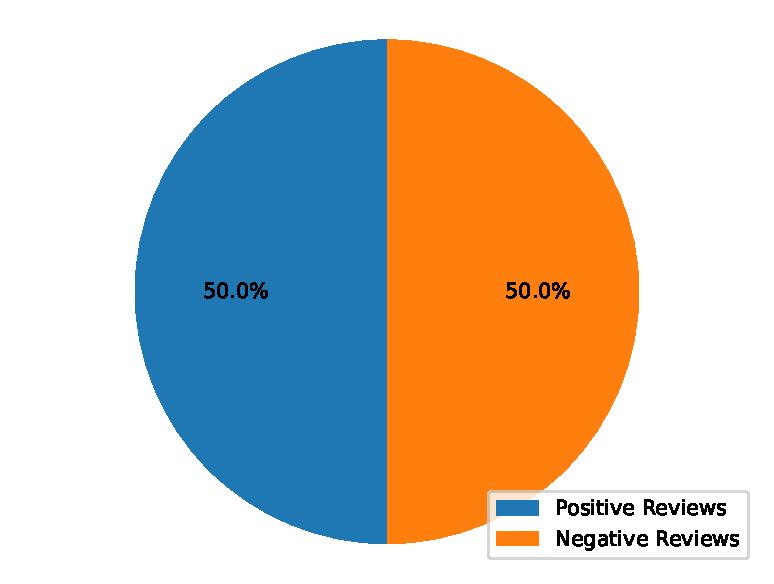
\includegraphics[width=\linewidth]{figures/train_labels.pdf}
        \caption{Distribution of Reviews' Labels}
        \label{fig:labels}
    \end{subfigure}
    %
    \begin{subfigure}{0.48\textwidth}
        \centering
        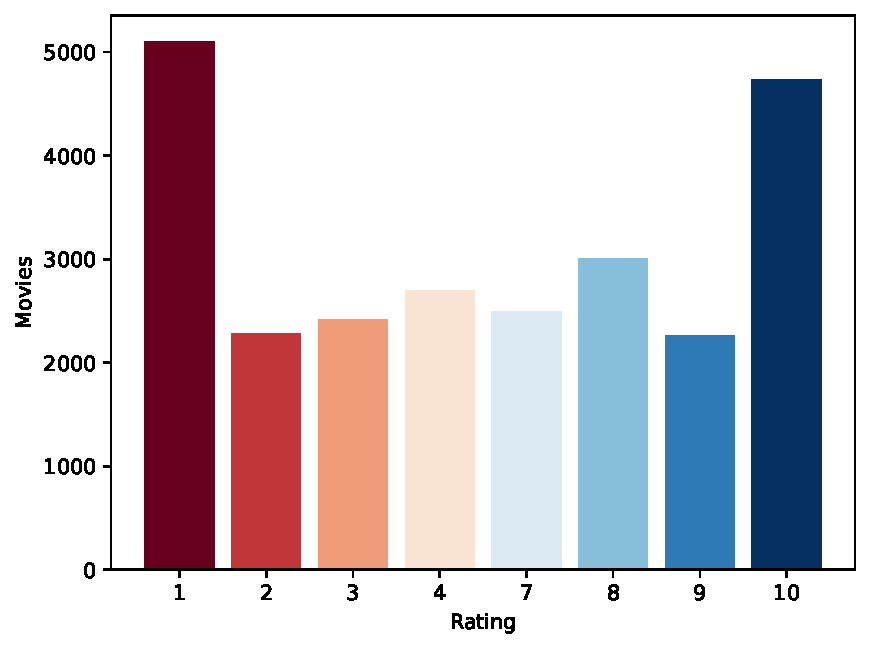
\includegraphics[width=\linewidth]{figures/train_ratings.pdf}
        \caption{Distribution of Movies' Ratings}
        \label{fig:ratings}
    \end{subfigure}

    \vspace{1cm}

    \begin{subfigure}{0.48\textwidth}
        \centering
        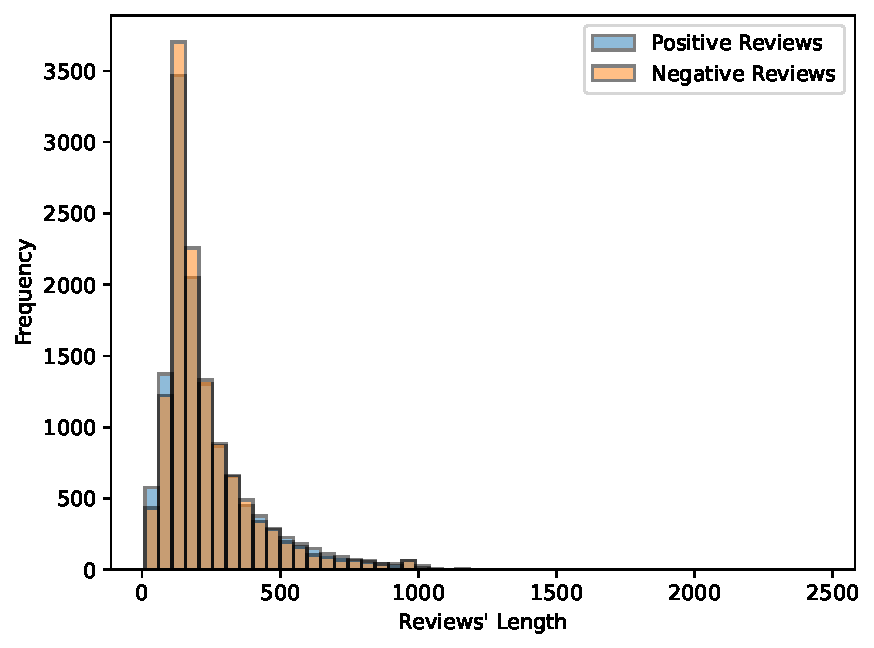
\includegraphics[width=\linewidth]{figures/train_lengths.pdf}
        \caption{Distribution of Reviews' Length (Words)}
        \label{fig:lengths}
    \end{subfigure}
    %
    \begin{subfigure}{0.48\textwidth}
        \centering
        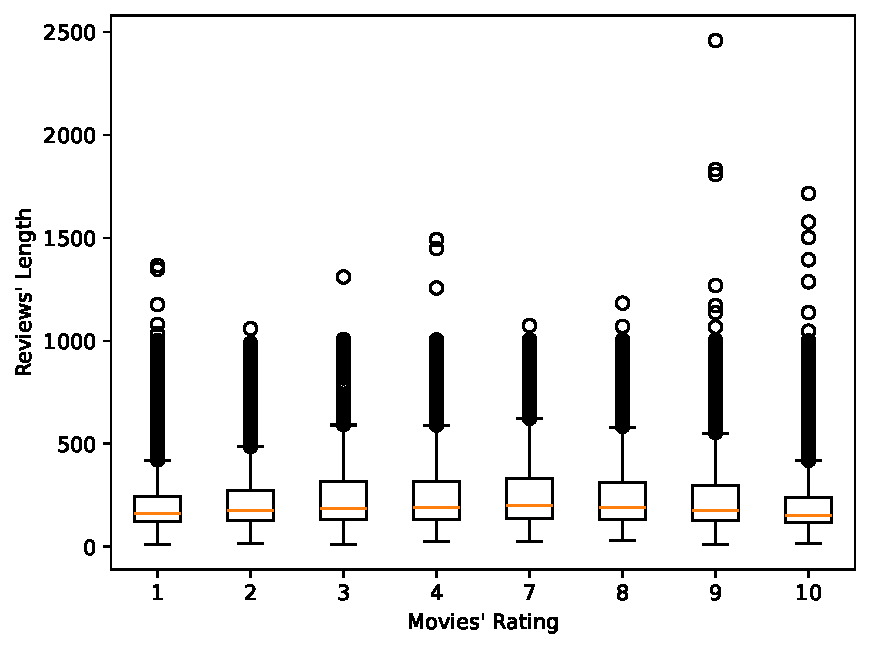
\includegraphics[width=\linewidth]{figures/train_lengths_ratings.pdf}
        \caption{Reviews' Length for Movies' Ratings}
        \label{fig:lengths_ratings}
    \end{subfigure}

    \caption{Exploratory Data Analysis of the IMDb Reviews Movie Dataset \cite{maas2011data}}
    \label{fig:descriptive}
\end{figure}


\section{Preprocessing}

To fully leverage the information embedded in the text of each review, effective preprocessing is an indispensable step. The objective of this stage in the pipeline is to filter out irrelevant information that introduces noise to the data, while retaining the distinctive characteristics of the text. From a technical point of view, the goal here is to extract a set of words from the text, which will be utilized in crafting an embedding for the review into a multidimensional space. This embedding serves as the input for any subsequent machine learning classifier. Let's briefly review the key steps undertaken in the preprocessing phase. The detailed steps of this preprocessing pipeline are outlined below:


\begin{enumerate}

    \item \textbf{Punctuation Removal:} The initial step involves eliminating punctuation marks from the text. This process ensures that only words are retained in the pipeline, as punctuation has a minor influence on the overall meaning of the sentence.

    \item \textbf{HTML Tag and URLs Removal:} This step focuses on stripping off all text with no specific semantic meaning. It includes the removal of HTML tags and any URLs mentioned in the reviews. Two distinct regular expressions are employed for this purpose.

    \item \textbf{Lowercasing:} Convert all words in the text to lowercase. This ensures uniformity among words and eliminates discrepancies arising from variations in casing, providing standardized input for subsequent processing.

    \item \textbf{Expansion of Contracted Forms:} 
    Expand contracted forms (e.g., "cannot" or "will not") and common slang forms (e.g., "going to" or "kind of") to their full forms. This step promotes consistency and is beneficial for the subsequent stopword removal step, as it brings back contracted words to their full form. Expansion is performed by checking words in the review against a handcrafted list from various web sources.

    \item \textbf{Stopword Removal:} Tokenize the text to work at the word level and remove common stopwords (e.g., "the," "and," "is"). This minimizes noise in the feature space, focusing the model on more meaningful content during sentiment analysis.

    \item \textbf{Stemming:} Implement stemming techniques to reduce words to their base or root form. Stemming involves removing prefixes or suffixes from words, aiming to capture the core meaning and consolidate variations. 

\end{enumerate}

This preprocessing pipeline is designed to refine and standardize textual data, establishing a robust foundation for the development of an effective text classifier. To illustrate, we present the transformation of the previous sample review through the preprocessing pipeline:


\begin{quote}
    \textit{['world', 'stage', 'people', 'actors', 'something', 'like', 'hell', 'said', 'theatre', 'stopped', 'orchestra', 'pit', 'even', 'theatre', 'door', 'audience', 'participants', 'theatrical', 'experience', 'including', 'story', 'film', 'grand', 'experiment', 'said', 'hey', 'story', 'needs', 'attention', 'needs', 'active', 'participation', 'sometimes', 'bring', 'story', 'sometimes', 'go', 'story', 'alas', 'one', 'listened', 'mean', 'said']
    }
\end{quote}

\section{Feature Extraction}
\label{sec:embeddings}

At this stage of the pipeline, once obtained a set of relevant words for each review, it becomes crucial to convert textual data into numerical vectors, enabling the application of mathematical operations and algorithms for the text classification task. In Natural Language Processing (NLP), two main approaches stand out: vector space models and word embeddings.


\subsection{Vector Space Models}

A Vector Space Model serves as a mathematical representation in natural language processing and information retrieval, portraying textual information. Documents or terms are depicted as vectors in a multi-dimensional space, with each dimension corresponding to a unique term in the dataset. These models form the basis for quantitatively analyzing textual data, facilitating efficient and scalable processing of large text corpora.


\subsubsection{Bag-of-Words (BoW)}

Within Vector Space Models, the Bag-of-Words (BoW) representation is fundamental. BoW disregards word order in a document, focusing solely on term frequency. It involves creating a vocabulary from unique terms in the dataset, representing each document as a vector. This vector's dimensions correspond to vocabulary terms, indicating term frequencies. Despite its simplicity, BoW is widely used in NLP due to its interpretability and ease of implementation.

Let $D$ be a document, $V$ the vocabulary, and $X_{\text{BoW}}$ the Bag-of-Words vector. $X_{\text{BoW}}(w_i)$ denotes the frequency of word $w_i$ in $D$:

\[
X_{\text{BoW}}(w_i) = \text{count}(w_i, D)
\]

Here, $\text{count}(w_i, D)$ represents the occurrences of $w_i$ in $D$.

\subsubsection{Term Frequency-Inverse Document Frequency (TF-IDF)}

BoW captures term frequency but neglects term importance in the corpus. TF-IDF addresses this by considering both term frequency and inverse document frequency, assigning higher weights to terms that are frequent in a document but rare in the corpus.

The Term Frequency (TF) of $w_i$ in $D$ is:

\[
\text{TF}(w_i, D) = \frac{\text{count}(w_i, D)}{\text{total words in } D}
\]

The Inverse Document Frequency (IDF) of $w_i$ in the corpus is:

\[
\text{IDF}(w_i, \text{corpus}) = \log\left(\frac{\text{total docs in corpus}}{\text{docs containing } w_i + 1}\right)
\]

The TF-IDF score for $w_i$ in $D$ is:

\[
\text{TF-IDF}(w_i, D, \text{corpus}) = \text{TF}(w_i, D) \times \text{IDF}(w_i, \text{corpus})
\]

The resulting TF-IDF scores form the TF-IDF vector $X_{\text{TF-IDF}}$ for $D$.












\subsection{Word Embeddings}

Word embeddings are dense vector representations that position words in a continuous vector space, capturing semantic relationships through their contextual usage. The features within this framework are latent features crafted by the model.
These embeddings play a crucial role in encapsulating the semantic meaning of words, enhancing our comprehension of language.
Nonetheless, an essential step is required to aggregate these word embeddings effectively in order to derive a comprehensive representation of a document. This aggregation process is imperative to transform individual word representations into a cohesive and meaningful portrayal of the entire document. In our approach, we will employ the average of all the word embeddings included in the review for this aggregation, ensuring a holistic representation.



\subsubsection{Word2Vec}

Word2Vec, abbreviated as Word to Vector, is a influential word embedding technique introduced by Google in 2013. Its significance lies in representing words as vectors in a continuous vector space, capturing semantic relationships. The algorithm employs two primary architectures: Skip-gram and Continuous Bag of Words (CBOW). Skip-gram predicts context words for a target word, adept at capturing linguistic nuances, while CBOW predicts a target word based on its context. Both architectures use a shallow neural network to produce embeddings.

One notable feature of Word2Vec is its ability to produce contextually rich representations for words, enabling the model to understand and generalize linguistic nuances. As a result, words with similar meanings end up with similar vector representations in the learned space. This property makes Word2Vec an effective tool for tasks such as word similarity, analogy completion, and even detecting semantic relationships between words.

In conclusion, Word2Vec has significantly shaped the landscape of NLP by providing a robust method for representing words in a way that preserves their semantic meaning.









\subsubsection{FastText}


FastText, developed by Facebook's AI Research (FAIR) lab in 2016, is a cutting-edge word embedding technique that builds upon the foundations laid by Word2Vec. This method extends the concept of word embeddings to include subword information, allowing it to capture morphological structures and handle out-of-vocabulary words more effectively.

At its core, FastText represents words as bags of character $n$-grams, where $n$ can range from individual characters to entire words. This subword information is crucial for handling morphologically rich languages and dealing with rare or unseen words. By considering subword units, FastText enhances its ability to represent the internal structure of words, making it adept at encoding morphological variations.

Similar to Word2Vec, FastText employs the Skip-gram model and the Continuous Bag of Words (CBOW) model. FastText, however, extends these architectures to operate on subword levels, contributing to its robustness in capturing intricate linguistic patterns.

FastText excels in scenarios where Word2Vec may struggle, such as handling rare words or morphologically complex languages. The ability to generate embeddings for subword units enables FastText to provide more informative representations, particularly useful in tasks like language modeling, text classification, and sentiment analysis.

A notable advantage of FastText lies in its capacity to generate embeddings for entire words based on their constituent subword units. This not only enhances performance on morphologically diverse languages but also facilitates the handling of previously unseen words during inference.



\section{Experimental Procedure}


After discussing and identifying important pre-processing steps for turning reviews into numerical data, we are ready to create a sentiment classification model for identifying sentiments in reviews.
Considering the limitations in time and resources, we have chosen a pipeline that prioritizes the efficient exploration of a diverse range of models and their respective parameter spaces, rather than delving deeply into the performance analysis of a single model.
The steps of our pipeline are the following:


\begin{enumerate}
    \item \textbf{Embedding Learning on Entire Training Set:} to begin, we performed embedding learning on our entire training dataset. This crucial step involved capturing the inherent representations of the data, thereby improving our capacity to extract meaningful patterns and features. For this process, we utilized one of the models outlined in Section~\ref{sec:embeddings}, focusing our tuning efforts solely on the number of features produced/retained in the output (see Table~\ref{tab:emb_params}).


    \item \textbf{Subsampling with Proportional Representation:} after the embedding phase, we conducted subsampling on the training set, considering a reduced portion (20\% of the dataset). This subsample maintained equal proportions of positive and negative reviews, aiming to create a subset that is representative of the entire dataset. The goal was to enable a more efficient training process across a diverse range of models and parameters.
        
    \item \textbf{Machine Learning Classifier Training with Grid Search:} the subsampled dataset was employed to train a machine learning classifier, choosing from three options: Logistic Regression, Naive Bayes, and SVM. To optimize their performance, we utilized a grid search approach, systematically exploring a predefined set of hyperparameters to identify the optimal configuration (see Table~\ref{tab:clf_params}). Furthermore, a 4-fold cross-validation strategy was implemented to robustly assess the model's performance across various subsets of the data. After the grid search, we pinpointed the top 5 models based on the average F1 Score across different folds. 

    \item \textbf{Final Model Training and Selection:} the top 5 models selected from the grid search were then trained on the entire original training set. This comprehensive training phase aimed to provide a more accurate representation of the models' capabilities on the complete dataset. Ultimately, we chose the best-performing model based on their F1 Scores obtained from the test set.

\end{enumerate}

We present the parameter grids used for the embedders and classifiers in Tables~\ref{tab:emb_params} and~\ref{tab:clf_params}. All parameters not explicitly mentioned were kept at their default values in the Python implementation.



\begin{table}[h]
    \centering
    \begin{tabular}{cc}
    \textbf{\begin{tabular}[c]{@{}c@{}}Bag-of-Words\\ TF-IDF\end{tabular}} & max\_features: {[}1000, 3000, 5000, 10000{]} \\ \hline
    \textbf{\begin{tabular}[c]{@{}c@{}}Word2Vec\\ FastText\end{tabular}}   & vector\_size: {[}100, 300, 500, 1000{]}
    \end{tabular}
    \caption{Grid search for embedders' parameters.}
    \label{tab:emb_params}
\end{table}



\begin{table}[h]
    \centering
    \begin{tabular}{cc}
    \textbf{Logistic Regression} & \begin{tabular}[c]{@{}c@{}}C: {[}0.1, 1, 10{]}\\ penalty: {[}"l1", "l2"{]}\end{tabular}                                       \\ \hline
    \textbf{SVM}                 & \begin{tabular}[c]{@{}c@{}}kernel: {[}'linear', 'rbf'{]}\\ C: {[}0.1, 1, 10{]}\\ gamma: {[}1, 'scale', 'auto'{]}\end{tabular} \\ \hline
    \textbf{Naive Bayes}         & \begin{tabular}[c]{@{}c@{}}alpha: {[}0.1, 1, 10{]}\\ fit\_prior: {[}False, True{]}\end{tabular}                              
    \end{tabular}
    \caption{Grid search for classifiers' parameters.}
    \label{tab:clf_params}
\end{table}
\section{Results}


In Table~\ref{tab:results}, we showcase the optimal results obtained by our models. To evaluate their performance, we furnish information about the optimal parameter combinations, accompanied by key metrics:

\begin{itemize}
    \item \textbf{Accuracy:} measure of the overall correctness of a classification model. It is calculated as the ratio of correctly predicted instances to the total instances.
    
    \item \textbf{Precision:} measure of the accuracy of the positive predictions made by a classification model. It calculates the ratio of correctly predicted positive observations to the total predicted positives.
    
    \item \textbf{Recall:} measure of the ability of a classification model to capture and correctly identify all the relevant instances. It calculates the ratio of correctly predicted positive observations to the total actual positives.
    
    \item \textbf{F1 Score:} harmonic mean of precision and recall, offering a balanced assessment that considers both false positives and false negatives.
    
\end{itemize}

In all these metrics we considered as positive label the "positive" rating. This comprehensive set of metrics offers a well-rounded assessment of our model's performance across various dimensions. Table~\ref{tab:results} summarize for each possible combination of embedder and classifier the best model obtained with the grid search.



\begin{table}[h]
    \centering
    \begin{tabular}{cccccc}
    \textbf{Model} & \textbf{Parameters}                                                                                & \textbf{Accuracy} & \textbf{Precision} & \textbf{Recall} & \textbf{F1 Score} \\ \hline
    T + LR    & \begin{tabular}[c]{@{}c@{}}max\_features: 10000\\ C: 1\\ penalty: l2\end{tabular}                  & 0.88              & 0.875              & 0.889           & 0.881             \\ \hline
    T + SVM   & \begin{tabular}[c]{@{}c@{}}max\_features: 10000\\ C: 10\\ gamma: scale\\ kernel: rbf\end{tabular}  & 0.878             & 0.883              & 0.871           & 0.877             \\ \hline
    BoW + SVM      & \begin{tabular}[c]{@{}c@{}}max\_features: 10000\\ C: 10\\ gamma: scale\\ kernel: rbf\end{tabular}  & 0.875             & 0.88               & 0.869           & 0.874             \\ \hline
    BoW + LR       & \begin{tabular}[c]{@{}c@{}}max\_features: 10000\\ C: 1\\ penalty: l2\end{tabular}                  & 0.867             & 0.864              & 0.871           & 0.868             \\ \hline
    T + NB    & \begin{tabular}[c]{@{}c@{}}max\_features: 5000\\ alpha: 1\\ fit\_prior: False\end{tabular}         & 0.837             & 0.86               & 0.806           & 0.832             \\ \hline
    BoW + NB       & \begin{tabular}[c]{@{}c@{}}max\_features: 5000\\ alpha: 1\\ fit\_prior: True\end{tabular}          & 0.837             & 0.86               & 0.805           & 0.832             \\ \hline
    W2V + SVM      & \begin{tabular}[c]{@{}c@{}}num\_features: 300\\ C: 10\\ gamma: 1\\ kernel: linear\end{tabular}     & 0.83              & 0.83               & 0.831           & 0.83              \\ \hline
    FT + SVM       & \begin{tabular}[c]{@{}c@{}}num\_features: 1000\\ C: 10\\ gamma: auto\\ kernel: linear\end{tabular} & 0.82              & 0.818              & 0.823           & 0.82              \\ \hline
    W2V + LR       & \begin{tabular}[c]{@{}c@{}}num\_features: 100\\ C: 0.1\\ penalty: l2\end{tabular}                  & 0.807             & 0.809              & 0.804           & 0.806             \\ \hline
    FT + LR        & \begin{tabular}[c]{@{}c@{}}num\_features: 300\\ C: 0.1\\ penalty: l2\end{tabular}                  & 0.806             & 0.807              & 0.804           & 0.805             \\ \hline
    \end{tabular}
    \caption{Best performance for each combination of embedder (T: TF-IDF, BoW: Bag of Words, W2V: Word2Vec, FT: FastText) and classifier (LR: Logistic Regression, SVM, NB: Naive Bayes).}
    \label{tab:results}
\end{table}


The obtained results demonstrate a robust generalization of all our models for this task, employing various techniques. This success can be attributed to the high quality of our pre-processing methods. The optimal approach for such tasks appears to involve a combination of a vector space model and a classification model, choosing between logistic regression and SVM. Despite training on the entire dataset, it appears that the corpus may not be sufficient to provide word embeddings with the necessary information to accurately represent the reviews.

To conclude our analysis, we futher analyze the performance of the best model in order to understand whether the errors are due to one of the general features of the reviews, or if it is mostly due to randomness.

To accomplish this, we computed the same distributions as presented in Section~\ref{sec:eda}, with a focus on highlighting the segment of data that has been misclassified. Figures~\ref{fig:pred_distro_ratings} and \ref{fig:pred_distro_length} depict the expected patterns from a well-generalizing model that exhibits no bias stemming from certain features.

Observing Figure~\ref{fig:pred_distro_ratings} and \ref{fig:pred_distro_length}, it becomes apparent that the model performs with higher accuracy on more extreme reviews, aligning with expectations and demonstrating proficiency in tasks that involve clear sentiment. However, as the rating approaches neutrality, the accuracy diminishes, indicating a potential need for further training to enhance performance to an even higher level. Importantly, this trend is consistent across reviews of varying lengths, suggesting that the model's performance remains stable and is not significantly influenced by the length of the reviews.

As a final verification step, we presented in Table~\ref{tab:logreg} the words associated with the highest coefficients in the Logistic Regression step. Examining these words allows us to confirm that the model has learned a set of terms that effectively represent either positive or negative sentiment, thereby equipping the model with a robust set of rules for accurately classifying reviews.



\begin{figure}[h]
    \begin{subfigure}{0.5\textwidth}
      \centering
      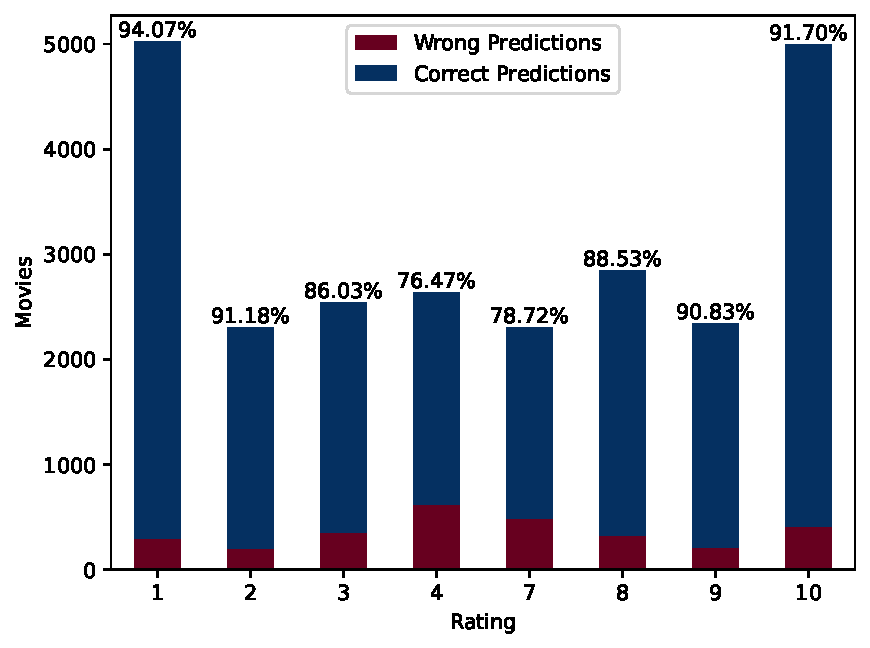
\includegraphics[width=\linewidth]{figures/t_lr_ratings.pdf}
      \caption{Predictions' distribution based on Ratings}
      \label{fig:pred_distro_ratings}
    \end{subfigure}%
    \begin{subfigure}{0.5\textwidth}
      \centering
      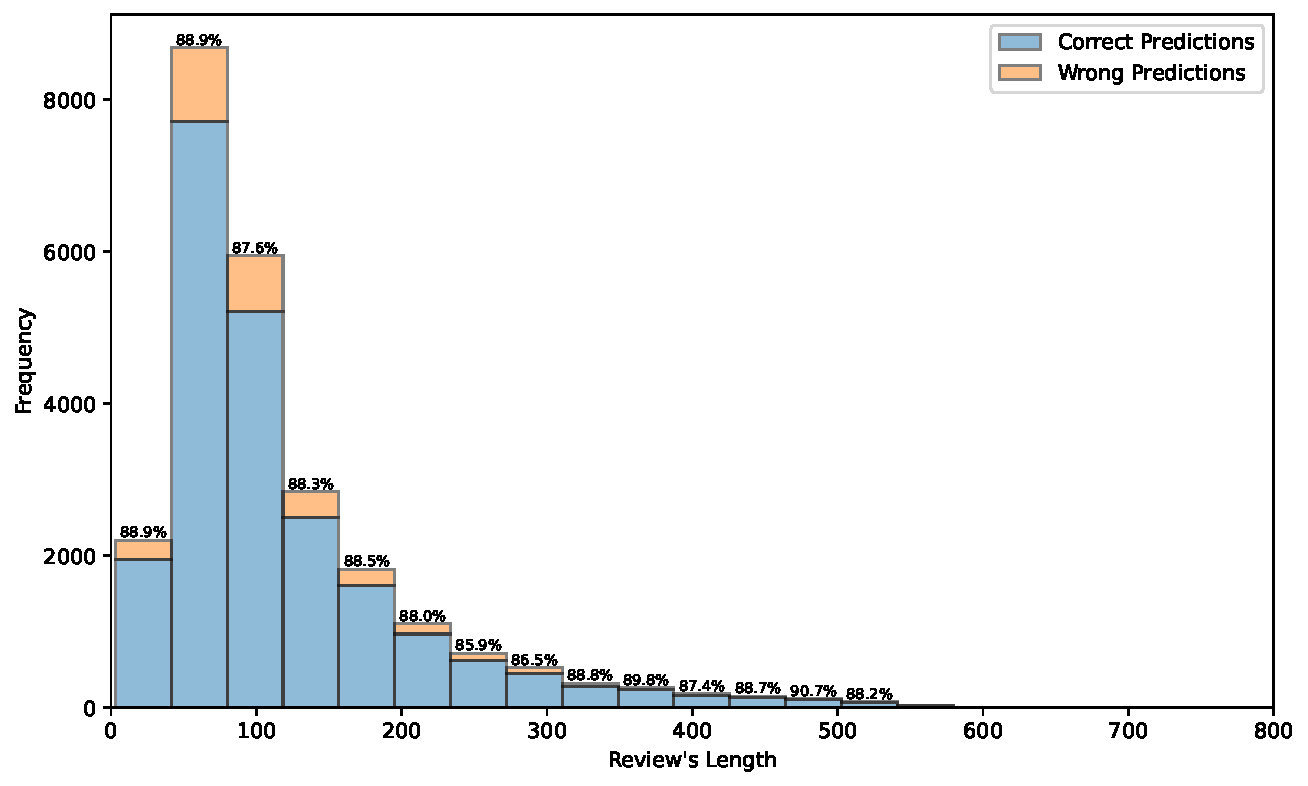
\includegraphics[width=\linewidth]{figures/t_lr_lengths.pdf}
      \caption{Predictions' distribution based on Reviews' length}
      \label{fig:pred_distro_length}
    \end{subfigure}
    \caption{}
  
  \end{figure}



\begin{table}[h]
    \centering
    \begin{tabular}{ccccc}
    \multicolumn{2}{c}{\textbf{Most "Positive" words}} &  & \multicolumn{2}{c}{\textbf{Most "Negative" words}} \\ \cline{1-2} \cline{4-5} 
    \multicolumn{1}{c|}{great}          & 6.519     &  & \multicolumn{1}{c|}{worst}            & -8.950  \\ \cline{1-2} \cline{4-5} 
    \multicolumn{1}{c|}{excellent}      & 5.974     &  & \multicolumn{1}{c|}{bad}              & -7.058  \\ \cline{1-2} \cline{4-5} 
    \multicolumn{1}{c|}{best}           & 4.933     &  & \multicolumn{1}{c|}{waste}            & -6.468  \\ \cline{1-2} \cline{4-5} 
    \multicolumn{1}{c|}{perfect}        & 4.732     &  & \multicolumn{1}{c|}{awful}            & -6.437  \\ \cline{1-2} \cline{4-5} 
    \multicolumn{1}{c|}{wonderful}      & 4.564     &  & \multicolumn{1}{c|}{boring}           & -5.642  \\ \cline{1-2} \cline{4-5} 
    \multicolumn{1}{c|}{amazing}        & 4.018     &  & \multicolumn{1}{c|}{poor}             & -5.177  \\ \cline{1-2} \cline{4-5} 
    \multicolumn{1}{c|}{favorite}       & 4.009     &  & \multicolumn{1}{c|}{nothing}          & -4.819  \\ \cline{1-2} \cline{4-5} 
    \multicolumn{1}{c|}{well}           & 3.824     &  & \multicolumn{1}{c|}{terrible}         & -4.621  \\ \cline{1-2} \cline{4-5} 
    \multicolumn{1}{c|}{loved}          & 3.655     &  & \multicolumn{1}{c|}{worse}            & -4.591  \\ \cline{1-2} \cline{4-5} 
    \multicolumn{1}{c|}{fun}            & 3.523     &  & \multicolumn{1}{c|}{poorly}           & -4.364  \\ \cline{1-2} \cline{4-5} 
    \multicolumn{1}{c|}{enjoyed}        & 3.516     &  & \multicolumn{1}{c|}{horrible}         & -4.283  \\ \cline{1-2} \cline{4-5} 
    \multicolumn{1}{c|}{love}           & 3.488     &  & \multicolumn{1}{c|}{dull}             & -4.186  \\ \cline{1-2} \cline{4-5} 
    \multicolumn{1}{c|}{highly}         & 3.479     &  & \multicolumn{1}{c|}{unfortunately}    & -4.043  \\ \cline{1-2} \cline{4-5} 
    \multicolumn{1}{c|}{today}          & 3.451     &  & \multicolumn{1}{c|}{disappointment}   & -4.043  \\ \cline{1-2} \cline{4-5} 
    \multicolumn{1}{c|}{superb}         & 3.285     &  & \multicolumn{1}{c|}{supposed}         & -3.839  \\ \cline{1-2} \cline{4-5} 
    \multicolumn{1}{c|}{brilliant}      & 3.281     &  & \multicolumn{1}{c|}{annoying}         & -3.791  \\ \cline{1-2} \cline{4-5} 
    \multicolumn{1}{c|}{definitely}     & 3.145     &  & \multicolumn{1}{c|}{disappointing}    & -3.681  \\ \cline{1-2} \cline{4-5} 
    \multicolumn{1}{c|}{enjoyable}      & 3.115     &  & \multicolumn{1}{c|}{ridiculous}       & -3.647  \\ \cline{1-2} \cline{4-5} 
    \multicolumn{1}{c|}{beautiful}      & 2.975     &  & \multicolumn{1}{c|}{fails}            & -3.635  \\ \cline{1-2} \cline{4-5} 
    \multicolumn{1}{c|}{fantastic}      & 2.965     &  & \multicolumn{1}{c|}{script}           & -3.616  \\ \cline{1-2} \cline{4-5} 
    \end{tabular}
    \caption{Words associated to largest coefficient in the Logistic Regression of the T+LR model.}
    \label{tab:logreg}
\end{table}
    









\bibliographystyle{plain}
\bibliography{biblio}


\end{document}
